\documentclass{article} % For LaTeX2e
\usepackage{cos424,times}
\usepackage{url}
\usepackage{graphicx}
\usepackage{hyperref}
\usepackage{caption}
\usepackage{subcaption}
\usepackage{amsmath}
\usepackage{amssymb}

\vbadness=10000

\title{Inferring Movie Characteristics from Dialogue}


\author{
Gregory McCord\\
Princeton University '20\\
\texttt{gmccord@princeton.edu} \\
}

\newcommand{\fix}{\marginpar{FIX}}
\newcommand{\new}{\marginpar{NEW}}

\begin{document}

\maketitle

\begin{abstract}

In the modern era, analysts use big data to predict outcomes and make decisions throughout different aspects of our lives. Now, algorithms are even being used to cast actors for movies and shows. The producers of the hit Netflix show \textit{House of Cards} cast Kevin Spacey as the protagonist based on the analysis of viewer preferences of an old British show by the same name \cite{hoc}. Someday perhaps, machine learning will even be used to generate movie scripts, but before this happens, it is imperative to understand if the set of words used in the dialogue of the movie correlates with properties of the movie itself. This study uses several methods to understand the properties of a movie using a bag-of-words representation of its dialogue to explore this paradigm. We used several labeled methods to predict well-defined characteristics of movies such as its genre(s) and year of production (older or younger). We also use an unlabeled method to infer the latent structure of each movie. We compared all classification methods using the misclassification rate and area under the receiver operating characteristic curve. For most cases of labeled prediction, the random forest classifier performed the best in terms of our evaluation metrics while logistic regression and naive bayes tended to perform equally well to each other. Latent dirichlet allocation helped us to understand the language of the movie outside of the bounds of typical forms of standard labeling methods in terms of language similarity between different genres while also demonstrating changes in the language in movies over time.

\end{abstract}

\section{Introduction}

Before machine learning can be used to aid in the generation of large bodies of text such as in the production of a movie script, researchers must first understand what lexicon should be used in the source corpora. That is, we must understand how the words used in a movie influence its characteristics so that they can be used in the prediction of the tastes of potential viewers. This study is significant because no prior research has attempted to draw inference for a movie's labeled or latent characteristics using only movie's script as the predictor. We tested three models for the labeled analysis of the dialogue. We used each model to predict our response variables - the era of production (old or new) and the genres. For the era of production, simple binary classification sufficed, but for predicting genres, we had to represent a movie's genres as a binary vector and treat each as a binary classification problem rather than as a single multiclass classification problem. As referenced before, we used logistic regression, naive bayes, and random forest models for this task. For the problem of unlabeled analysis, we used latent dirichlet allocation to better understand how the scripts of different genres, producers, and eras interacted. In this paper, we will first discuss related work examples before describing our methods in depth, followed by a discussion and analysis of all results of the study.

\section{Related Work}

While our approach to analyzing a movie's characteristics based solely on the vocabulary used in the movie is novel, several other studies have attempted to analyze scripts in different ways. One such study, from the University of London, attempts to analyze the structure of the narrative in scripts \cite{film1}. Another study treats scripts as unstructured text in an effort to reveal patterns in the narrative through the use of sentiment analysis \cite{film2}. Both of these papers indicate that there is potential for understanding the structure of the movie, but neither explores the vocabulary used in the movies or the influences of genres on the analysis of the scripts.

\section{Methods}

\subsection{Data Overview}

We obtained the data as a dataset from the Kaggle website. The data was originally generated by Cornell University researchers for the purpose of comparing the structure of dialogue in movies to that of real world communication. The data contains dialogue excerpts from 617 movies from a variety of decades (as far back as the 1930s and as recent as the 2000s). There are 220,579 unique conversations involving over 9,000 characters. Although the corpus of movies is relatively small, it still provides over 300,000 total sentences for analysis. \cite{kaggle}

The dataset also contains additional metadata that aids in our classification. Each movie has its year of production, a list of its genres, and several IMDb statistics including the user rating and number of votes. While the IMDb statistics could be very interesting to investigate to see if the vocabulary used in a movie influences the reviews it receives, this study focuses on the use of the first two components.

\subsection{Data Processing}

The original files received from the Kaggle website were tab-delimited and contained every line of dialogue in addition to the movie, character, and line number. Additionally, some of the movie scripts contained tabs or special characters in their dialogue. We built a simple Regular Expression to capture the desired fields and remove the intractable characters. We then combined the lines of dialogue into a script for each movie and converted it into a DataFrame.

Then we created the bag of words representation of the data in several steps. First, we used the Python NLTK library to tokenize, lemmatize, and stem using the porter method to treat the data (the code for this step was adapted from that of assignment 1). We then iterated over the scripts to create a universal vocabulary of the scripts, which contained over 11,000 root words. We then created a matrix containing the word counts for each movie. Finally, we normalized these counts over the total number of words contained in the script of the movie. We did not perform manual feature selection - instead we allowed the regularization of the models to perform feature selection innately.

With respect to the metadata, we needed to turn the list of genres into a usable form. As such, we used a binary genre vector to extract the binary response variables for each movie with respect to all genres. In the end, there were 23 genres, but several of these had low numbers of counts and were excluded from the model creating process further into the experiment.

\subsection{Analysis Methods}

We used several methods for analyzing the data. For the purpose of binary classification, we used 3 classification models from the scikit-learn Python library \cite{skl}. We used 5-fold cross validation in order to tune the hyperparameters of the corresponding models for each binary response variable. As addressed before, although genre classification at first glance appears to be a multiclass problem, it truly is a multilabel classification problem instead since most movies are tagged with multiple genres. To combat this, we used the binary relevance approach combined with a binary vector of the genre response variables to iterate over the genre list and generate a different model with a binary response variable for each genre. We also used built-in scikit-learn methods to split the data into a 70:30 training:testing split that we maintained for all models and iterations. The methods used were as follows:
\begin{enumerate}
\item \textit{Logistic Regression with $\ell_2$ penalty}
\item \textit{Naive Bayes classifier}: using the multinomial implementation
\item \textit{Random Forest}: using gini impurity scores
\end{enumerate}

Additionally, we used latent dirichlet allocation with 5 topics to analyze the latent structure. We used a gensim Python wrapper for the MALLET implementation of the algorithm \cite{mallet} \cite{gensim}. In order to use this, we had to convert the bag of words matrix into a sparse list of words and their paired counts for each document. We used this representation without normalizing the feature counts for the corpus as input to the algorithm and received in response 2 lists. The first contains each movie with a probability distribution over the possible topics while the second contains a breakdown of the topic as a linear combination of the influential features and their corresponding weights. We manually interpreted the results for this method in order to discover trends in our classification methods while also understanding the latent structure of the topics and movies, which is not normally captured by typical categorizations such as genre.

We felt all of these methods helped reveal different features of the structure of the scripts. We used LDA because it felt like a natural approach for analyzing the latent topic structures of the movies given a bag of words representation of the movie. For the labeled methods, naive bayes is always a reasonable choice for a baseline model for classification because of its primary assumption - that the features are independent. Similarly, logistic regression is a good baseline model because it helps determine if the data is linearly separable or not - while we did not expect this to be the case, it is an important possibility to verify. Finally, the random forest model is a powerful nonlinear classifier that seemed to be likely to succeed where logistic regression and naive bayes failed.

\subsection{Evaluation of Results}

To evaluate the results of our labeled classification for all response variables (for the era and each genre), we used two different metrics on the out of sample movies. Our primary method was the misclassification rate:
\begin{align*}
MC_j = 1 - \frac{TP_j}{TP_j + FP_j}
\end{align*}

where $MC_j$ is the misclassification rate of the $j^{th}$ response variable and $TP_j$ and $FP_j$ are count variables representing the number of true positives and false positives, respectively, for the specific response variable. Additionally, we used the receiver operating characteristic curve - more specifically the area under the curve - which has the added benefit of determining how sensitive our models are to changes in the threshold value. The ROC curve compares the true positive rate with the false positive rate, which are defined as follows:
\begin{align*}
TPR_j = \frac{TP_j}{TP_j + FN_j} \hspace{5mm} FPR_j = \frac{FP_j}{FP_j + TN_j}
\end{align*}

where $TN_j$ and $FN_j$ are defined similarly as above except as the counts of true negatives and false negatives.

\section{Results and Discussion}

Now we will explore the results of our analysis. First we will observe the results of the era classification before moving onto the genre classification. We will conclude the results section with the analysis of the LDA results.

\subsection{Era Classification} \label{era}

When classifying movies as either old or new, there are several things to consider - most importantly, we had to determine what years determined the bounds of 'new' and 'old'. Rather than perform grid search to determine which set of bounds provided the best bounds, we tested several reasonable bounds and reported the findings of several combinations. Notably, we tested bounds such that no movies were excluded (that is, the upper boundary for 'old' was adjacent to the lower boundary for 'new') and those that excluded some movies. In Figure \ref{year_data}, the columns 'Low Year' and 'High Year' refer to these boundaries. Similarly, the columns 'Number Old Movies' and 'Number New Movies' refer to the number of movies (out of the 617 total) that are labeled as 0 (Old) and 1 (New) - movies produced in years outside these bounds were excluded from this classification task.

\begin{figure}[htb]
\centering
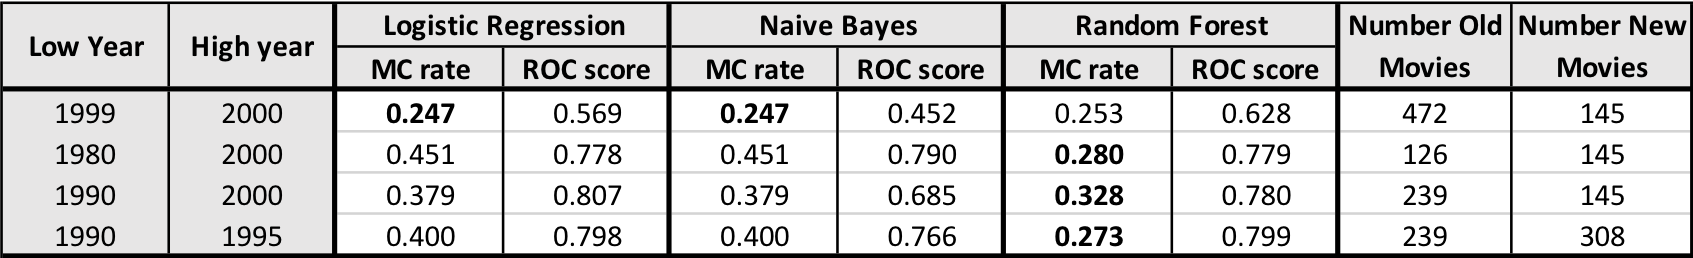
\includegraphics[width=1\linewidth]{year}
\caption{Era Classification results}
\label{year_data}
\end{figure}

It is clear that both Naive Bayes and Logistic Regression performed relatively poorly in this classification task. Despite the strong performance of those same models on the data when using a narrow bound, namely where low = 1999 and high = 2000, we ultimately determined that the success of the model came from the fact that there was such a large difference in the sample sizes for 'old' versus 'new' based on that boundary set. The data seems to indicate that the linear classifiers struggled to classify the data, indicating that it is perhaps a task better suited to clustering or decision trees. The result most indicative of this result is when the bounds were set to low = 1990 and high = 2000 and the movie counts on each side of the partition were close together. The random forest model performed very well, especially when compared with the linear classifiers.

When we use the Gini impurity scores for each feature as generated by the random forest model, we can map their indices back to our vocabulary list and observe the most influential terms for the era classification problem. Several of the top terms were 'everyone', 'someone', 'shit', and 'girlfriend'. At first glance, these terms seem more like a coincidence than anything, but by using the Google Books Ngram Viewer tool, we are able to compare the usage of a word in published works over time. For all four of these terms, the percent-usage has more than doubled from 1980 to 2000. Further, 'shit' and 'girlfriend' are recorded in nearly 0 works prior to 1970, demonstrating that this discrepancy seen in books is likely to have manifested itself in the scripts of movies, helping nonlinear classifiers accurately predict whether movies are old or young based solely on the vocabulary used.

\subsection{Genre Classification}

Similar to classification for era, we treated each response variable (genre) independently, even if a movie was labeled as multiple genres. As a result, for genres that tend to occur together such as action and adventure, the results can begin to resemble each other more so than they would if we considered all possible combinations of genres - that is, 'action', 'adventure', and 'action and adventure'. However, the results indicate that, in general, this is a safe assumption to make. We did not generate models for genres with low counts. It was not clear what the cutoff point should be, but we ultimately continued our research with the top 10 of the 23 represented genres, the results of which are displayed in Figure \ref{genre_data}.

For an unknown reason, logistic regression and naive bayes achieved identical classification rates for all of the displayed genres. However, when you compare the methods using the ROC score, logistic regression outperformed naive bayes in most cases. As before though, random forest outperformed these classification methods. Surprisingly still is that there are several genres such as horror and romance where the results among all models were comparable. It appears that for these genres in particular, linearly separable models perform as well as nonlinear methods. There are two cases where the linear models perform poorly as compared to the random forest classifier - drama and thriller. Our analysis of these genres indicates that there was a great deal of overlap between these genres and several of the other genres. Particularly, 'drama' seemed to be an umbrella term for many movies with over half of the 617 movies possessing that label while 'thriller' was often paired with either horror or crime. In both cases, we believe that the broad scope and high levels of overlap made the data difficult to linearly separate.

\begin{figure}[htb]
\centering
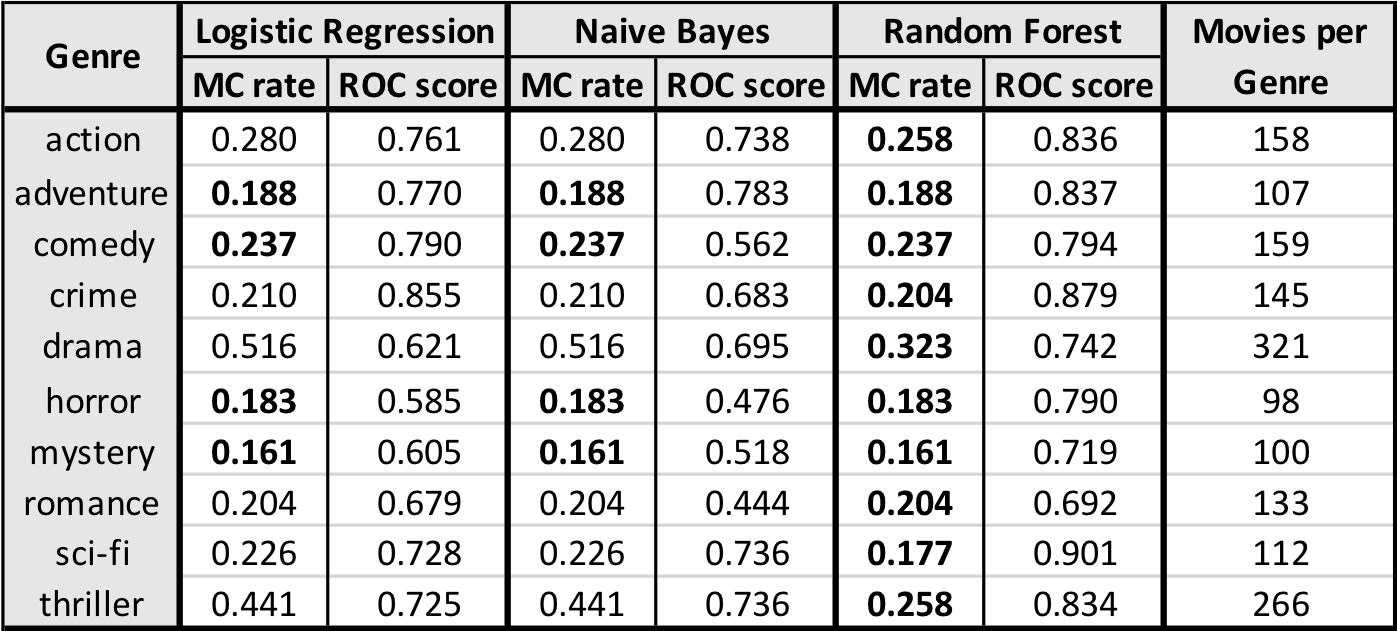
\includegraphics[width=0.8\linewidth]{genre} 
\caption{Genre Classification results}
\label{genre_data}
\end{figure}

Next, we generated a confusion matrix on the whole dataset to understand which genres were commonly being mistook for others, which can be found in Figure \ref{confusion_data}. This data was generated using the random forest classifier. An important detail to note is that each row sum is greater than 1. This is because, for a confusion matrix generated from multi-labeled data, each movie or data point is counted multiple times unlike in multiclass classification. As a result, each cell in the table represents the fraction of movies of the $i^{th}$ genre that are classified as the $j^{th}$ genre where $i$ and $j$ represent the row and column indices, respectively. This does not indicate that the results are flawed or that many movies are misclassified but rather that a large percentage of movies have a pattern of multiple labels, and this trend can witnessed by seeing large fractions of movies of one genre being classified as another.

\begin{figure}[htb]
\centering
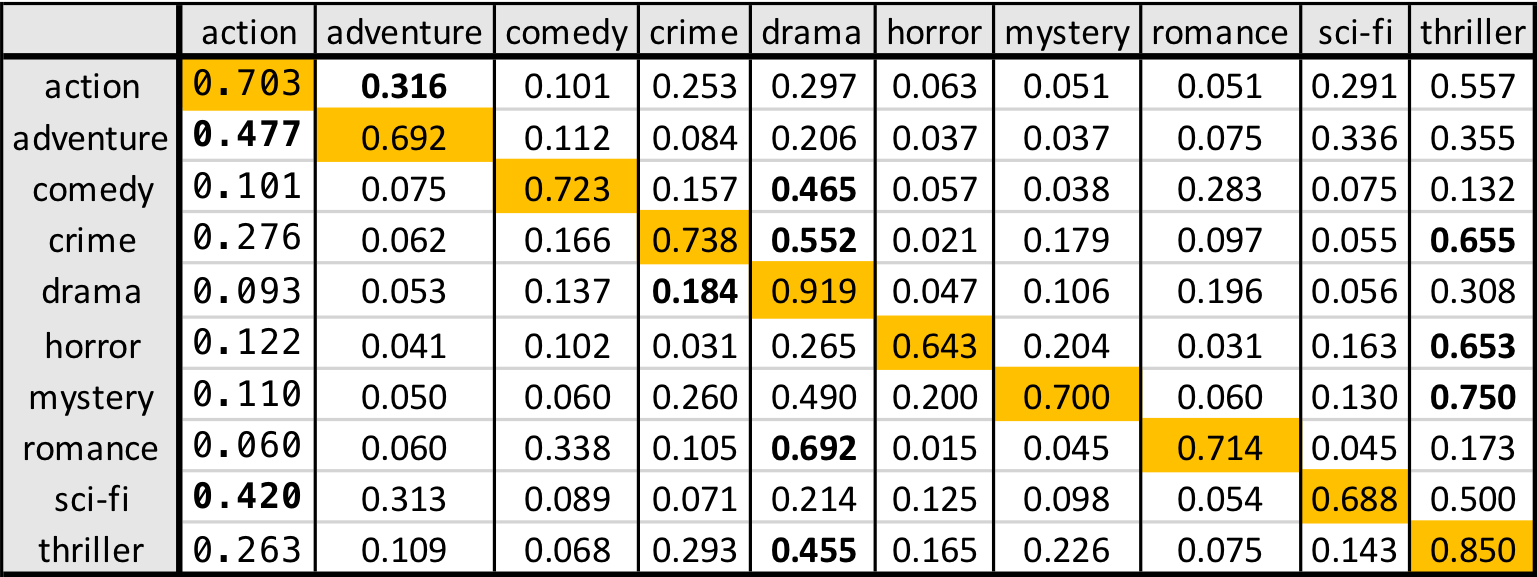
\includegraphics[width=0.8\linewidth]{confusion} 
\caption{Genre Confusion Matrix}
\label{confusion_data}
\end{figure}

We have highlighted the major diagonal to indicate that movies that are a certain genre have a high chance of being correctly classified as that genre. Several other interesting values have been indicated as well. An interesting insight is the property that the matrix need not be symmetric, and this especially shows up in the confusion results for crime and drama. The results seem to indicate that crime movies are commonly also labeled as dramas but that dramas are less commonly crime fighting movies. Simply based on the fact that drama is a broad label, this result cognitively makes sense, but the corpus from Cornell verifies our hypothesis. Of the 617 movies, 145 are labeled crime, 321 are labeled drama, and 78 are labeled as both. However, both in the corpus and in our predictions, it is interesting to note that not many movies are classified as both mystery and crime despite their seemingly high degree of similarity.

From here, we begin our analysis of the influential terms in each of these genres. As before, we determined these features by using a random forest model with tuned hyperparameters and sorted them by gini impurity score. While we were unable to find patterns in the terms of the genre comedy - likely because humans do not think of comedy in terms of a bag of vocabulary words but rather as a structured jokes - the terms in most cases painted a clear picture of how the models determined one movie genre from another. The results may be seen in Figure \ref{term_data}.

\begin{figure}[htb]
\centering
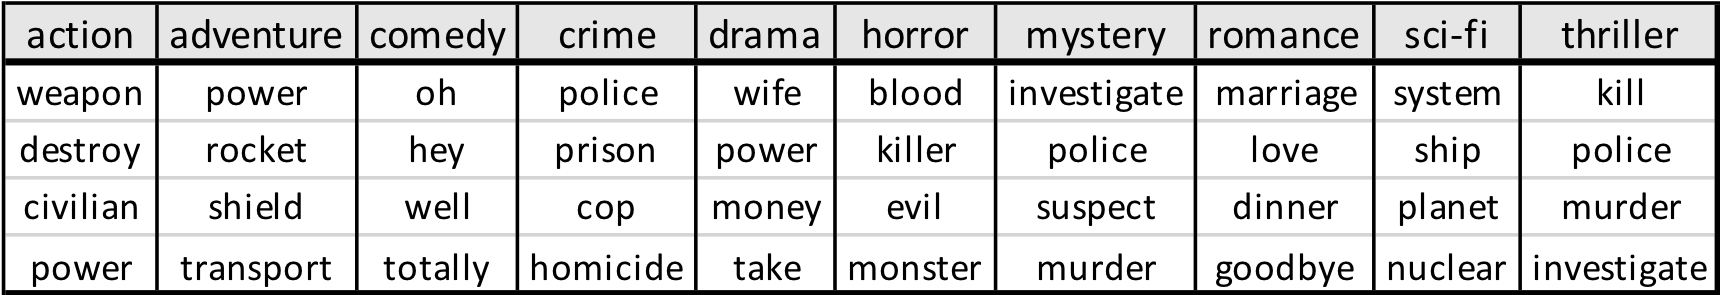
\includegraphics[width=1\linewidth]{terms}
\caption{Influential Terms by Genre}
\label{term_data}
\end{figure}

Just by observing the list of words under each category, we can already begin to see natural overlap between genres. For instance, crime and mystery movies both contain high percentages of words dealing with police or investigations, as we might expect given the nature of the two genres. An interesting point to note is that the word 'power' appears in action, adventure, and drama, even though drama does not appear to be closely related to the other two genres. This is a case where using a unigram bag-of-words model misses context and therefore could misclassify movies as a result. Typically in the sense of a drama, the word 'power' means political sway whereas in the case of an action or adventure movie, power tends to refer to strength. On the other side, we can easily understand that action and adventure would both be dependent on the word 'power' since the two genres tend to overlap in many movies. Another point to note is that thriller overlaps many genres so cleanly that all of its top terms are shared by other genres. Our classification results indicated this overlap, but the similarity of the top terms solidifies our hypothesis. However, it is interesting to note that despite the disparity between crime and mystery according to our prior analysis, the two genres appear to have several similar top terms. From the other top terms for these genres (not shown in the chart), it appears as though crime movies have stronger, more active terms associate with them such as 'kill', 'shot', or 'dealer' whereas mystery movies use more passive imagery like 'investigate','case', and 'statement'.

Finally, we selected several interesting cases to explore further by plotting the ROC curves. These curves may be seen in Figure \ref{roc_data}.

\begin{figure}[htb]
\centering
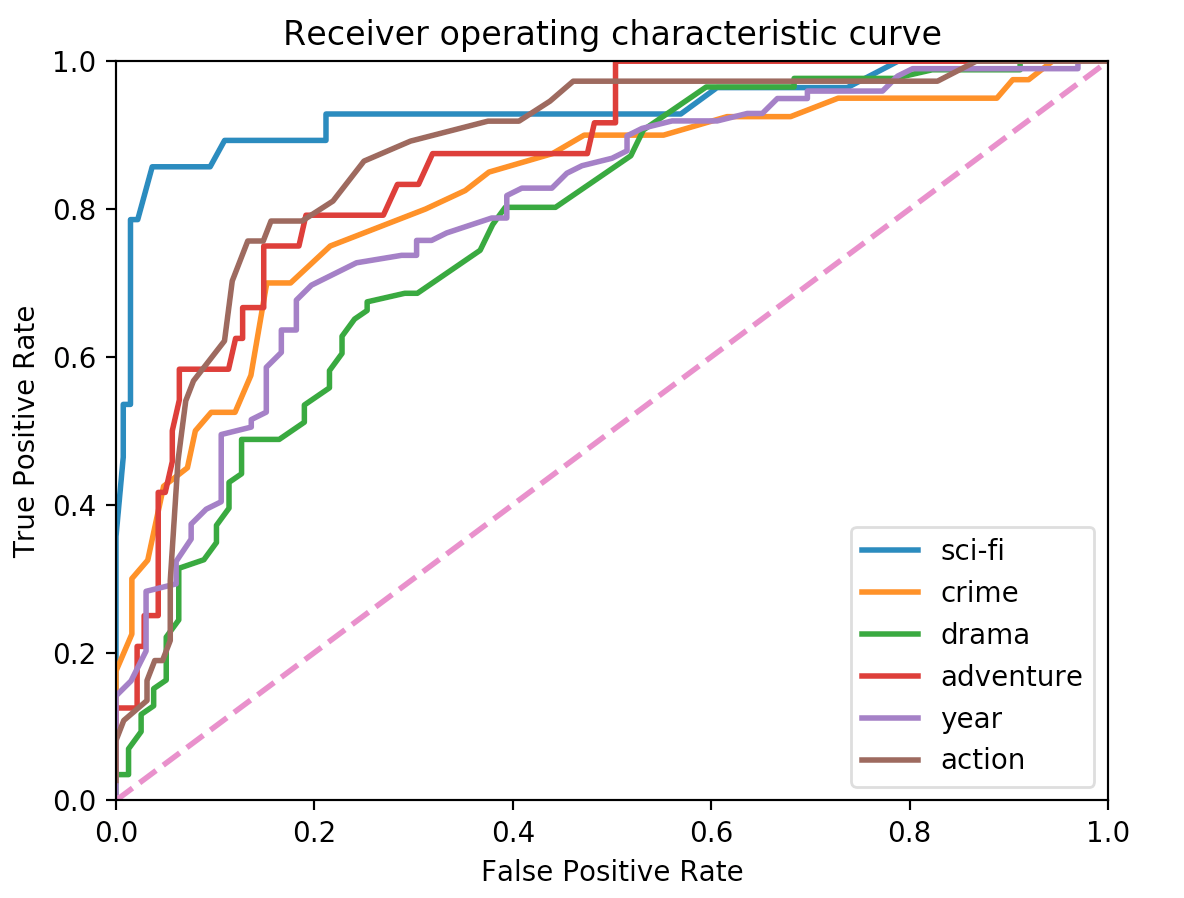
\includegraphics[width=0.8\linewidth]{roc}
\caption{ROC curve for Binary Classification Tasks from the Random Forest Model}
\label{roc_data}
\end{figure}

We included 5 genres - action, adventure, crime, drama, and sci-fi - as well as the era classification for comparison. We were interested in seeing how efficiently the model could classify a movie as given its vocabulary, and the results tended to match what we expected. The easiest movies for the random forest model to classify appear to be sci-fi movies, likely due to the fact that they have a very conserved lexicon including terms such as 'system' and 'ship' as shown before. Although not all sci-fi movies have these specific terms, those that do were easy for the model to classify accurately. Most of the other categories seemed to be relatively consistent in how certain the model was in its classification. As expected, action and adventure lined up very closely given the similarity of the language used in each. The model however was less certain in its classification of drama movies since it is a broad topic. We expect individual terms to have less overall impact on the prediction rather than in the case of sci-fi where certain words are highly correlated with the genre.

\subsection{Latent Topic Analysis}

Now that we have concluded our analysis of our binary classification models, we will analyze the latent topics generated by the LDA algorithm with 5 topics. We tested the model both with 5 and 10 topics and many random seeds but ultimately decided that the 5 topic model generated stronger results. While increasing the number of topics allows for more separation between different types of movies, we felt that discovering how the latent structures of the movies interacted provided more valuable insight. Our results can be found in Figure \ref{lda_data}. There are 4 sets of rows - the first set is the set of genres that had very high percent topic scores for that specific topic, the second contains interesting trends that were external to the genres, and the last two are self-explanatory.

\begin{figure}[htb]
\centering
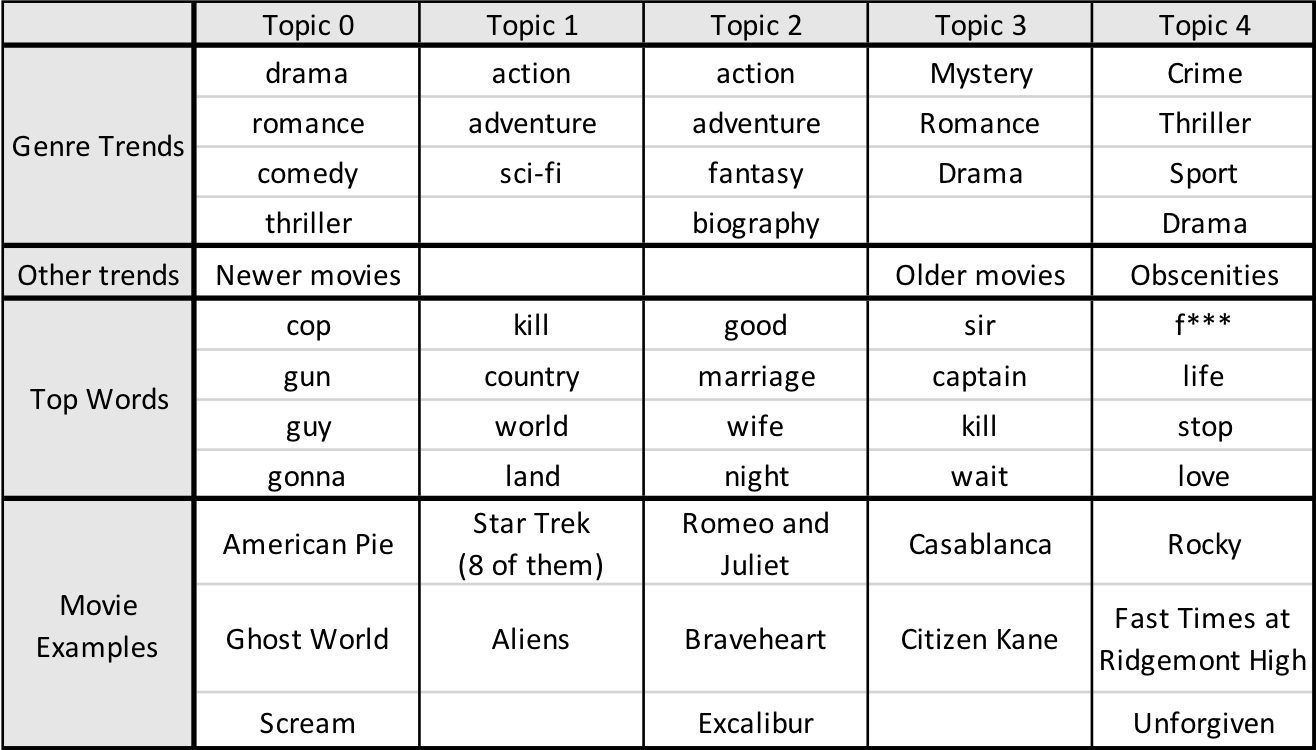
\includegraphics[width=0.8\linewidth]{lda} 
\caption{Analysis of Latent Topic Model with 5 Topics}
\label{lda_data}
\end{figure}
 
At first glance, most of the genre groupings make intuitive sense and have already been touched on in earlier parts of this analysis. That being said, the other trends realized by the model add more depth to these topics. By comparing the movies labeled in topic 0 and topic 3, we realized that most of the movies with high proportions of topic 3 were produced in the pre-1980 era, going as far back as 1932, while many movies in topic 0 were produced in the late 1990s and 2000s. Using the Google Ngram Viewer, we compared the usage of the top terms over the decades and noticed that 'guy' and 'gonna' from topic 0 had doubled between 1980 and 2000 while the usage of 'sir' and 'captain' from topic 3 had been cut in half. There are obvious outliers however, the most likely of which are those like \textit{Titantic} which were made in recent times but are set years ago. Another interesting trend was spotted in topic 4, whose top words included a great deal of profanity. Despite this however, many of the movies that correlated strongly with this topic like \textit{Rocky} were not rated R and therefore contained no profanity. Our analysis showed that many of these movies contained violence and strong language. As such, although it did not contain obscenities, it contained the same style of language as many action/sport/thrillers. For the opposite reason however, \textit{Fast Times at Ridgemont High} (an R rated comedy/drama) had a high proportion of topic 4 despite having little violence.
 
Observing the final two sets of rows, we see more results that confirm our prior hypotheses. The influential terms in each topic correlate well with the proposed labels for the topic and the influential terms seen in our labeled analysis of genres. The movie examples serve only to reaffirm our prior analysis. One final point is the consistency of the movies listed in topic 1 - of the top 10, 8 of them were Star Trek movies. This further goes to show that our topic model seems to be discerning reasonable topics since a sci-fi series oftentimes has a fairly conserved vocabulary. In other topics, we witnessed similar results like the \textit{Ghostbusters} and \textit{Airplane!} series.

\section{Conclusion}

We began this study intending to discover if there was any relationship between the vocabulary used in a given movie and any characteristics that we can tell about it. When we began analyzing the results using our baseline models, the results did not indicate a strong correlation - in several cases, logistic regression and naive bayes performed barely better than a random classifier. However, once we introduced the random forest classifier, we began to see strong results across the board, indicating that the predicting genre from a vocabulary set is not a linearly separable task. We analyzed our genre and era classification results by examining influential terms and the genre confusion matrix. The results of this analysis bolstered our confidence in our random forest model despite our initial skepticism given the nature of the classification task at hand. Finally, this led us to using LDA to understand the latent structure of the movies, which we believed would lead us to unique topic groupings that transcended the typical genre classification scheme. Ultimately, the LDA algorithm accomplished this task - it reinforced our results from binary classification but also revealed trends in obscenities and language over time, which we had not expected would be important features when finding differences in the vocabulary sets used in each topic.

Based on the success of our classifiers and the inference gained from the analysis of latent topics, we believe that movie characteristics can be predicted using strictly the vocabulary contained in the movie. Due to the success of the random forest model, we believe that future analysis of movie genres using a bag-of-words representation of the script could also implement K-means clustering or K-nearest neighbor classification. Additionally, the analysis of the corpus using higher numbers of topics for the LDA algorithm could lead to discoveries on interesting differences that cause separation among similar genres, rather than an analysis more focused on the similarities that existed, which is more prevalent in a topic model with 5 topics. Further, the original corpus contained metadata for other possible response variables including the number of votes and the voter score (the popularity of the movie and how well it was received), which could lead to an interesting analysis of predicting viewer response from the words in the script. Finally, the most valuable extension to this project would be an extended corpus containing more movies from all decades, particularly the 2000s and 2010s, allowing researchers to train these models on bigger datasets. We believe that this is a successful first step in using machine learning to understand and interpret movie dialogue and, potentially, someday in the generation of scripts.

\bibliography{ref}
\bibliographystyle{plain}

\end{document}
